Σε αυτό το κεφάλαιο παρουσιάζουμε τα αποτελέσματα για την collective επικοινωνία για τις αρχιτεκτονικές NUMA και UMA. Θα παρουσιάσουμε τα αποτελέσματα για μερικά από τα collectives ξεχωριστά παραλείποντας τα collectives που έχουν παρόμοιες υλοποιήσεις. Συγκεκριμένα, θα περιοριστούμε στην αναλυτική παρουσίαση των \textit{scatter}, \textit{bcast} και \textit{allreduce} και στο τέλος θα παραθέσουμε συνοπτικά τα αποτελέσματα για τα υπόλοιπα collectives.  Για όλα τα collectives αναπτύσσεται κοινό μοντέλο επικοινωνίας. Ωστόσο, για την βελτίωση των αποτελεσμάτων προσθέσαμε στα χαρακτηριστικά ένα tag, που αντιπροσωπεύει το collective, έτσι ώστε το μοντέλο μας να μπορεί να ξεχωρίσει το τύπο collective που προσπαθούσαμε να προβλέψουμε. Μπορούσαμε ισοδύναμα, να εκπαιδεύσουμε ξεχωριστά μοντέλα για κάθε τύπο collective αλλά θεωρήσαμε την επιλογή μας πιο εύχρηστη. Στο τέλος του κεφαλαίου παραθέτουμε επίσης, τις προβλέψεις για το collective \textit{allreduce} που χρησιμοποιεί η εφαρμογή LULESH.

\section{Scatter}
\paragraph{}
Ξεκινώντας από την UMA αρχιτεκτονική, στο Σχήμα \ref{fig:scatter_sizes} φαίνονται οι προβλέψεις για το collective scatter με σταθερό μέγεθος\footnote{Σε όλες τις περιπτώσεις με το μέγεθος αναφερόμαστε στο μήκος των κομματιών που σπάει ο μεγάλος buffer εισόδου} και διάφορους ζητούμενους πόρους. Σημειώνουμε ότι, σε αυτές τις προβλέψεις το training και το testing set ήταν τα ίδια. Σκοπός μας ήταν να αξιολογήσουμε κατά πόσο το μοντέλο καταφέρνει με το training set , που βασίζεται στο αφηρημένο communication pattern που αναπτύξαμε, να δώσει ρεαλιστικές προβλέψεις (self-validation) . Από τα αποτελέσματα παρατηρούμε ότι, αν εξαιρέσουμε κάποια ελάχιστα σφάλματα για τα μηνύματα μεγέθους 1KiB, το μοντέλο προβλέπει σωστά τους χρόνους επικοινωνίας. 
\paragraph{}
Επίσης, ενδιαφέρον έχει και ο τρόπος που ο χρόνος επικοινωνίας κλιμακώνει. Για μέγεθος 1KiB και PPN 4,6 και 8 η επικοινωνία κλιμακώνει. Το working set του benchmark χωράει στην κρυφή μνήμη, με την επικοινωνία να μην επηρεάζεται καθόλου από τη κύρια μνήμη και να εκμεταλλεύεται πλήρως το ψηλό bandwidth του διαδρόμου. Για τα δύο επόμενα μεγέθη ο χρόνος επικοινωνίας αυξάνει σχετικά γραμμικά με την αύξηση των πόρων.  Αντίθετα για το μεγαλύτερο μήνυμα που εξετάσαμε, 1MiB, παρατηρούμε μη γραμμική αύξηση στο χρόνο επικοινωνίας καθώς ο μεγάλος όγκος των δεδομένων πιέζει όλο και περισσότερα τμήματα της αρχιτεκτονικής του συστήματος. Ωστόσο, ο μεγαλύτερος χρόνος επικοινωνίας παραμένει μικρότερος από 4ms.
\paragraph{}
Επιπλέον, στο Σχήμα \ref{fig:scatter_conf} φαίνονται οι χρόνοι και οι προβλέψεις για κάποια configu\-rations και όλα τα μεγέθη μηνυμάτων που εξετάσαμε. Σε αναλογία με το προηγούμενο σχήμα, το μοντέλο μας καταφέρνει να κάνει ακριβείς προβλέψεις. Αυτό που ξεχωρίζει από το σχήμα είναι ότι ο χρόνος επικοινωνίας για τα μηνύματα μήκους μικρότερου από 2KiB είναι σχετικά σταθερός. Μετά από μια απότομη μεταβολή στους χρόνους από τα 2KiB στα 4KiB ο χρόνος ξεκινά και αυξάνει με το μέγεθος του μηνύματος.
\begin{figure}[H]
    \centering
    \captionsetup{justification=centering,margin=0cm}
    \begin{subfigure}[b]{0.45\textwidth}
        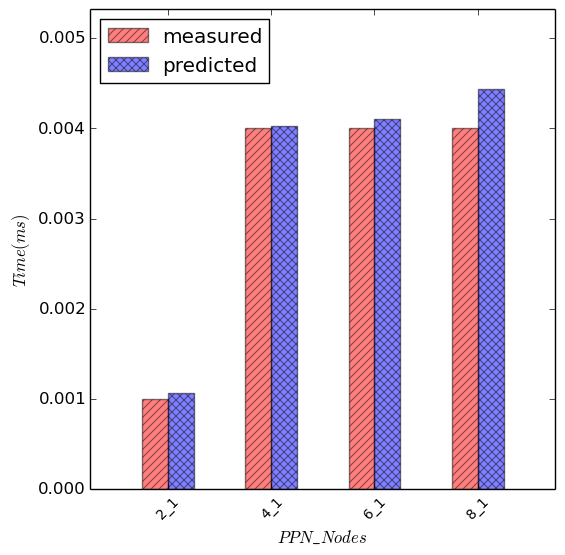
\includegraphics[width=\textwidth]{./images/scatter/scatter_1024}
        \caption{1KiB}
    \end{subfigure}
    \quad 
        \begin{subfigure}[b]{0.45\textwidth}
        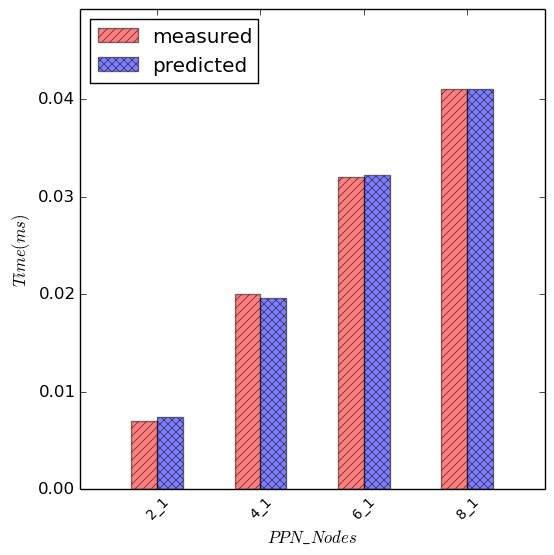
\includegraphics[width=\textwidth]{./images/scatter/scatter_16384}
        \caption{16KiB}
    \end{subfigure}
    \quad
        \begin{subfigure}[b]{0.45\textwidth}
        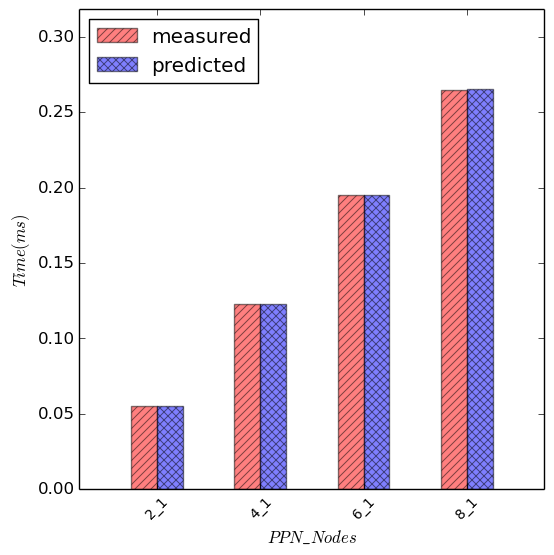
\includegraphics[width=\textwidth]{./images/scatter/scatter_262144}
        \caption{256KiB}
    \end{subfigure}
    \quad
        \begin{subfigure}[b]{0.45\textwidth}
        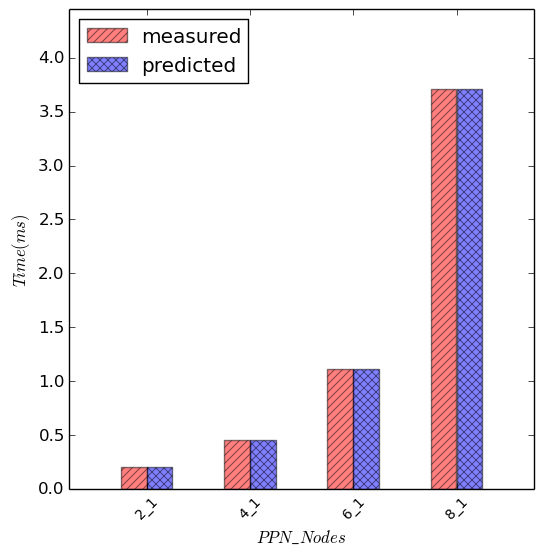
\includegraphics[width=\textwidth]{./images/scatter/scatter_1048576}
        \caption{1MiB}
    \end{subfigure}

    \caption{Αποτελέσματα scatter για σταθερό μέγεθος μηνύματος σε αρχιτεκτονική UMA}
        \label{fig:scatter_sizes}
\end{figure}
\begin{figure}[H]
    \centering
    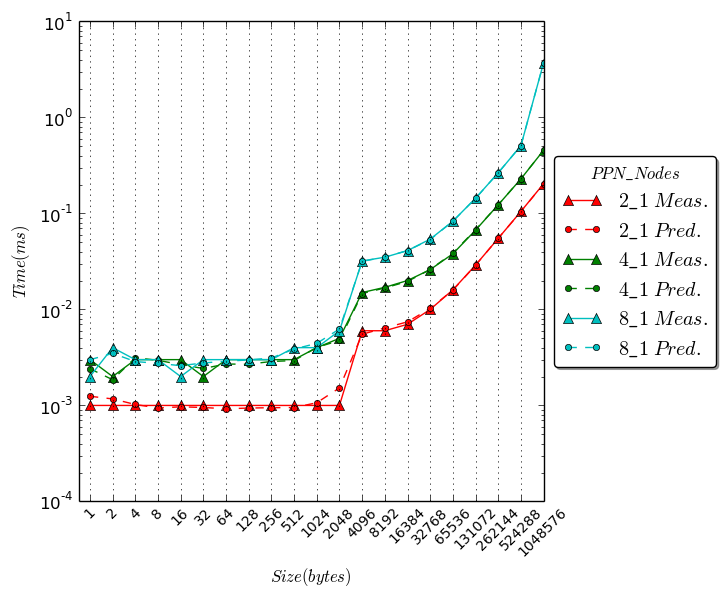
\includegraphics[width=0.65\textwidth]{./images/scatter/scatter.png}
    \caption{Αποτελέσματα scatter για μερικά configurations σε αρχιτεκτονική UMA}
    \label{fig:scatter_conf}
\end{figure}


\paragraph{}
Όπως και για την UMA αρχιτεκτονική, στο Σχήμα \ref{fig:scatter_sizes_NUMA} δίνονται οι προβλέψεις για σταθερός μήκος μηνύματος και μεταβαλλόμενο μέγεθος των δεσμευμένων πόρων, ενώ στο Σχήμα \ref{fig:scatter_conf_NUMA} δίνονται οι προβλέψεις για όλα τα μεγέθη μηνύματος και για μερικά configurations. Η γενική εικόνα σχετικά με τις προβλέψεις παραμένει η ίδια, με το μοντέλο μας να επιδεικνύει πολύ καλή συμπεριφορά. Σε αντιδιαστολή με την αρχιτεκτονική UMA, παρατηρούμε αύξηση στο χρόνο επικοινωνίας και για μικρότερα μεγέθη μηνύματος. Τα αποτελέσματα για τα configurations \textit{8\_2} και \textit{4\_4} είναι αρκετά κοντά, με την επικοινωνία πάνω από πρώτο να διαρκεί ελάχιστα περισσότερο χρόνο για μηνύματα μεγαλύτερα από 256B και το δεύτερο να υπερέχει για τα μικρότερα. Φαίνεται, ότι για τα μικρότερα μηνύματα, η επικοινωνία εκμεταλλεύεται τη κοντινή απόσταση μεταξύ των MPI διεργασιών και το configuration με τα περισσότερα PPN είναι γρηγορότερο. Στην αντίθετη περίπτωση, το δίκτυο διασύνδεσης των κόμβων μπορεί να διαχειριστεί καλύτερα τα μεγαλύτερα μηνύματα και έτσι υπερέχει της πρώτης. 

\begin{figure}[ht]
    \centering
    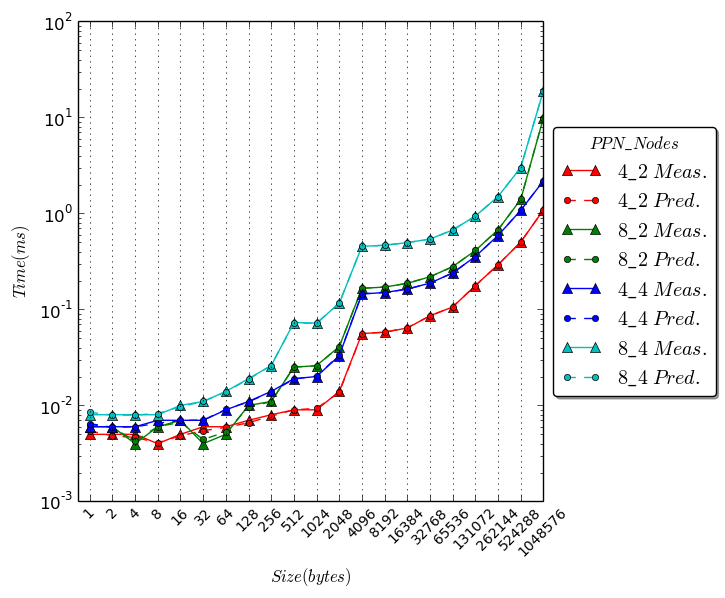
\includegraphics[width=0.7\textwidth]{./images/scatter_NUMA/scatter.png}
    \caption{Αποτελέσματα scatter για μερικά configurations σε αρχιτεκτονική NUMA}
    \label{fig:scatter_conf_NUMA}
\end{figure}

\begin{figure}[H]
    \centering
    \captionsetup{justification=centering,margin=0cm,font=footnotesize}
    \begin{subfigure}[b]{0.4\textwidth}
        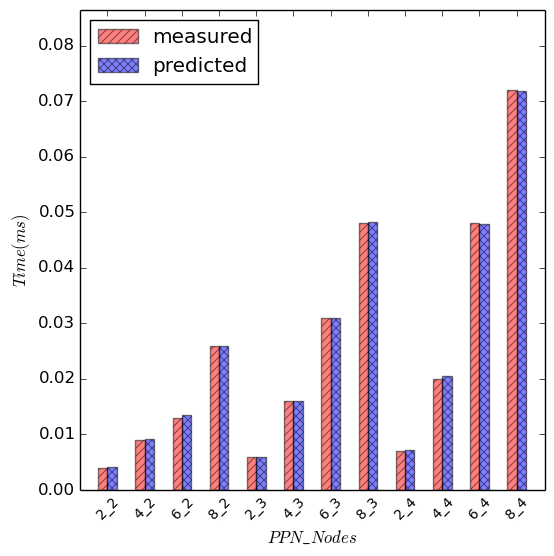
\includegraphics[width=\textwidth]{./images/scatter_NUMA/scatter_1024}
        \caption{1KiB}
    \end{subfigure}
    \quad 
        \begin{subfigure}[b]{0.4\textwidth}
        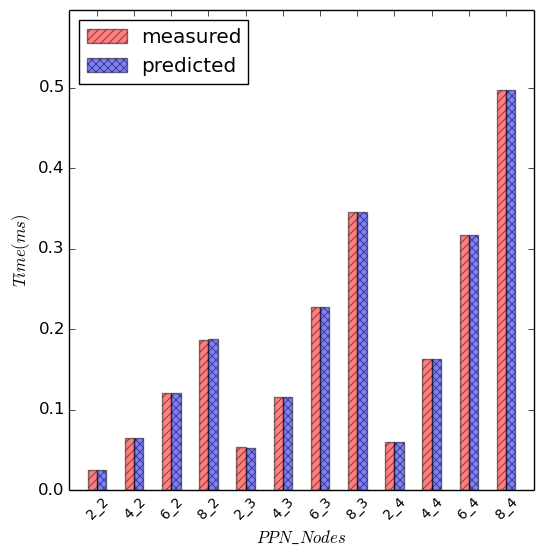
\includegraphics[width=\textwidth]{./images/scatter_NUMA/scatter_16384}
        \caption{16KiB}
    \end{subfigure}
    \quad
        \begin{subfigure}[b]{0.4\textwidth}
        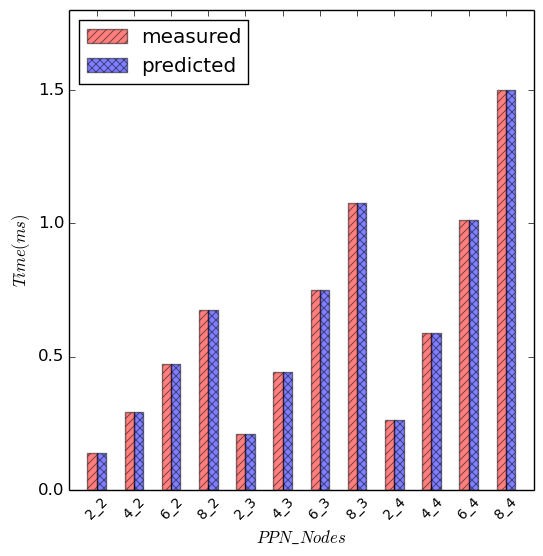
\includegraphics[width=\textwidth]{./images/scatter_NUMA/scatter_262144}
        \caption{256KiB}
    \end{subfigure}
    \quad
        \begin{subfigure}[b]{0.4\textwidth}
        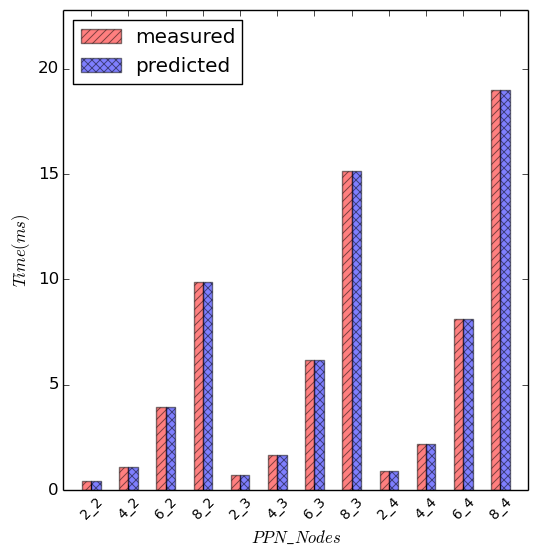
\includegraphics[width=\textwidth]{./images/scatter_NUMA/scatter_1048576}
        \caption{1MiB}
    \end{subfigure}

    \caption{Αποτελέσματα scatter για σταθερό μέγεθος μηνύματος σε αρχιτεκτονική NUMA}
        \label{fig:scatter_sizes_NUMA}
\end{figure}



%\section{Gather}
%Συνεχίζοντας, στα Σχήματα \ref{fig:gather_sizes} και \ref{fig:gather_conf} παραθέτουμε τα αποτελέσματα για το collective gather σε αρχιτεκτονική UMA ενώ στα Σχήματα \ref{fig:gather_sizes_NUMA} και \ref{fig:gather_conf_NUMA} δίνονται τα αντίστοιχα γραφήματα σε NUMA αρχιτεκτονική. Όσο αφορά την UMA αρχιτε το μικρότερο μήνυμα, μεγέθους 8Β, παρατηρήσαμε κάποιου περίεργη συμπεριφορά με το χρόνο για 8 πυρήνες να είναι μικρότερος από το χρόνο που απαιτείται για 6 διεργασίες. Ωστόσο, η διαφορά μεταξύ τους είναι μόλις  1us κάνοντας τη ακριβή διερεύνηση των αιτιών πίσω από το φαινόμενο αδύνατη. Τα μεγαλύτερα μηνύματα εμφανίζουν πιο κανονική συμπεριφορά. Καθώς η απότομη αύξηση στο χρόνο επικοινωνίας όταν το μέγεθος του μηνύματος αυξάνεται από 2KiB σε 4KiB εμφανίζεται και σε αυτό το collective, ερευνήσαμε περισσότερο την αιτία που το προκαλεί. Τελικά, τα 4KiB είναι το ελάχιστο μέγεθος όπου εφαρμόζεται το KNEM, προσθέτοντας το overhead που αναφέραμε στο Κεφάλαιο της εισαγωγής. Αυτός είναι και ο λόγος της απότομης μεταβολής του χρόνου για τα συγκεκριμένα μεγέθη. 
%
%\begin{figure}[H]
%    \centering
%    \captionsetup{justification=centering,margin=0cm}
%    \begin{subfigure}[b]{0.45\textwidth}
%        \includegraphics[width=\textwidth]{./images/gather/gather_8.png}
%        \caption{8B}
%    \end{subfigure}
%    \quad 
%        \begin{subfigure}[b]{0.45\textwidth}
%        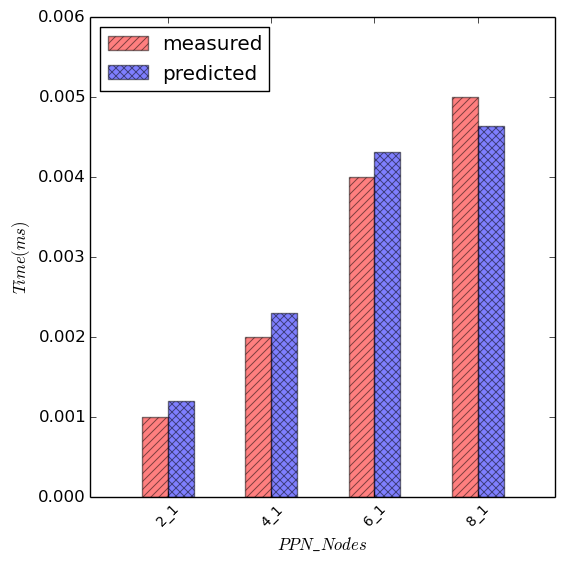
\includegraphics[width=\textwidth]{./images/gather/gather_1024.png}
%        \caption{1KiB}
%    \end{subfigure}
%    \quad
%        \begin{subfigure}[b]{0.45\textwidth}
%        \includegraphics[width=\textwidth]{./images/gather/gather_4096.png}
%        \caption{4KiB}
%    \end{subfigure}
%    \quad
%        \begin{subfigure}[b]{0.45\textwidth}
%        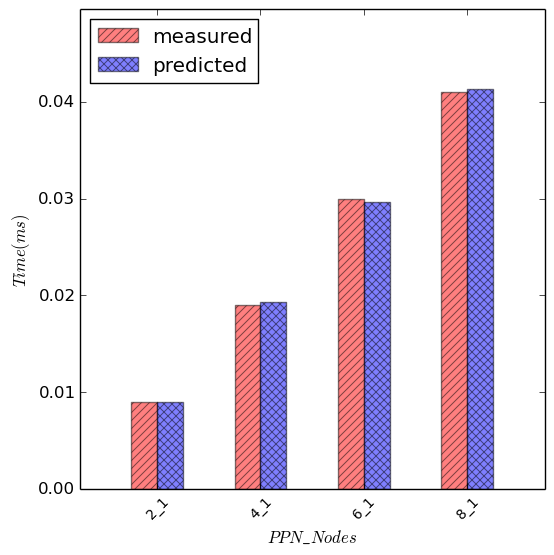
\includegraphics[width=\textwidth]{./images/gather/gather_16384}
%        \caption{16KiB}
%    \end{subfigure}
%
%    \caption{Αποτελέσματα gather για σταθερό μέγεθος μηνύματος σε αρχιτεκτονική UMA}
%        \label{fig:gather_sizes}
%\end{figure}
%
%\begin{figure}[H]
%    \centering
%    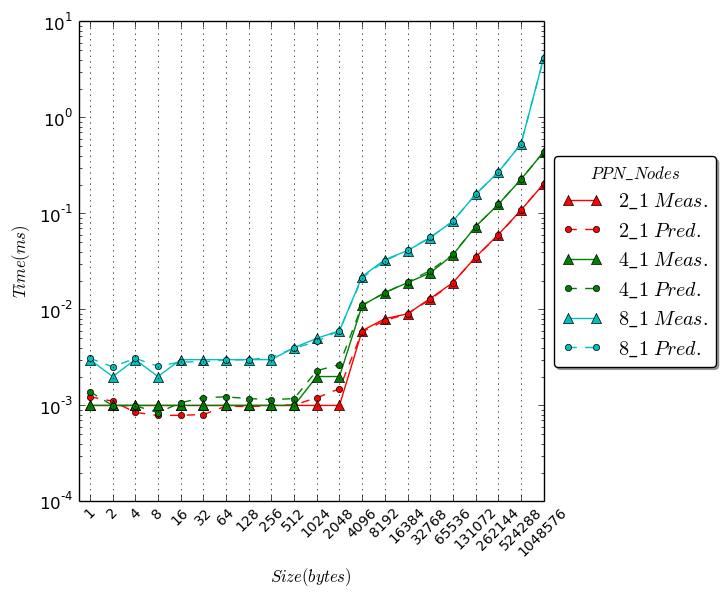
\includegraphics[width=0.65\textwidth]{./images/gather/gather.png}
%    \caption{Αποτελέσματα gather για μερικά configurations σε αρχιτεκτονική UMA}
%    \label{fig:gather_conf}
%\end{figure}
%
%\begin{figure}[H]
%    \centering
%    \captionsetup{justification=centering,margin=0cm}
%    \begin{subfigure}[b]{0.45\textwidth}
%        \includegraphics[width=\textwidth]{./images/gather_NUMA/gather_8.png}
%        \caption{8B}
%    \end{subfigure}
%    \quad 
%        \begin{subfigure}[b]{0.45\textwidth}
%        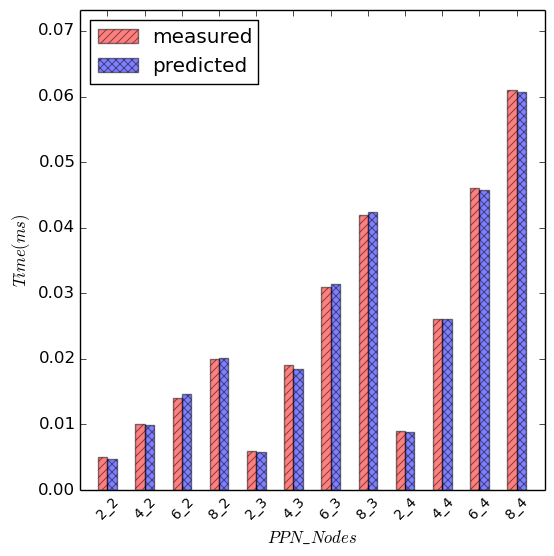
\includegraphics[width=\textwidth]{./images/gather_NUMA/gather_1024.png}
%        \caption{1KiB}
%    \end{subfigure}
%    \quad
%        \begin{subfigure}[b]{0.45\textwidth}
%        \includegraphics[width=\textwidth]{./images/gather_NUMA/gather_4096.png}
%        \caption{4KiB}
%    \end{subfigure}
%    \quad
%        \begin{subfigure}[b]{0.45\textwidth}
%        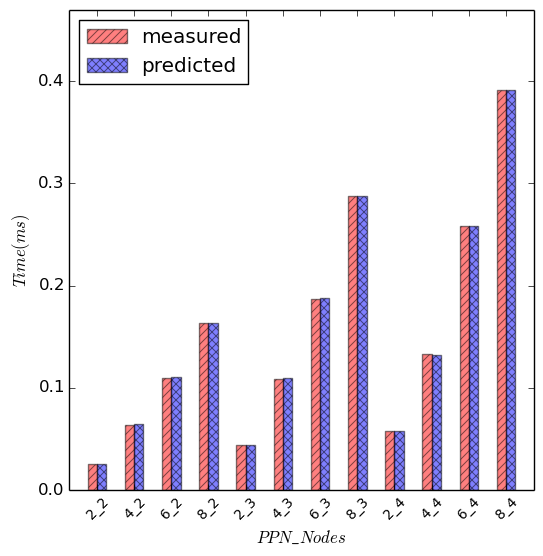
\includegraphics[width=\textwidth]{./images/gather_NUMA/gather_16384}
%        \caption{16KiB}
%    \end{subfigure}
%
%    \caption{Αποτελέσματα gather για σταθερό μέγεθος μηνύματος σε αρχιτεκτονική NUMA}
%        \label{fig:gather_sizes}
%\end{figure}
%
%\begin{figure}[H]
%    \centering
%    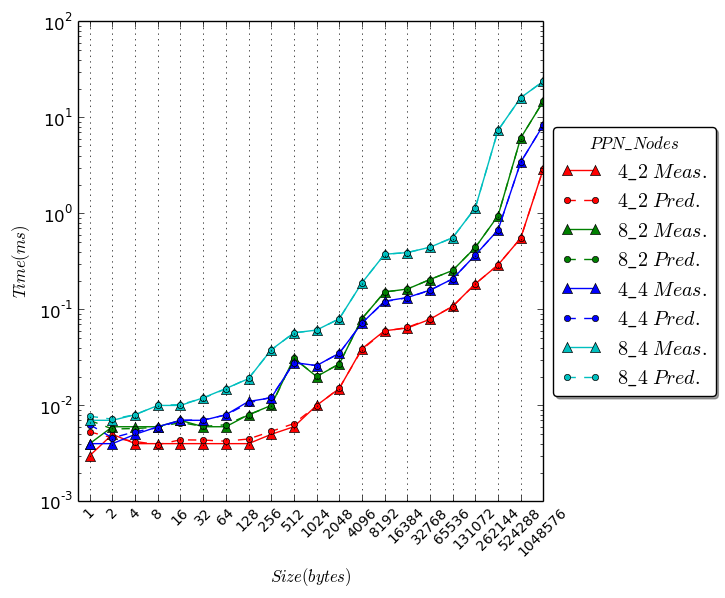
\includegraphics[width=0.65\textwidth]{./images/gather_NUMA/gather.png}
%    \caption{Αποτελέσματα gather για μερικά configurations σε αρχιτεκτονική NUMA}
%    \label{fig:gather_conf}
%\end{figure}

\section{Broadcast}
Συνεχίζοντας, στα Σχήματα \ref{fig:bcast_sizes} και \ref{fig:bcast_conf} παραθέτουμε τα αποτελέσματα για το collective bcast σε αρχιτεκτονική UMA ενώ στα Σχήματα \ref{fig:bcast_sizes_NUMA} και \ref{fig:bcast_conf_NUMA} δίνονται τα αντίστοιχα γραφήματα σε NUMA αρχιτεκτονική. Σε όλες τις προβλέψεις η ακρίβεια είναι ικανοποιητική με ελάχιστα σφάλματα, και πάλι, για τα μικρότερα μεγέθη μηνυμάτων. Η συμπεριφορά του broadcast εμφανίζει δύο μεγάλες διαφορές από το scatter. Αρχικά, δεν έχουμε απότομη αύξηση στο χρόνο επικοινωνίας με τη μετάβαση από 2KiB σε 4KiB για καμία από τις δύο αρχιτεκτονικές. Επιπλέον, φαίνεται ότι η μεταβολή του χρόνου καθώς οι δεσμευμένοι πόροι αυξάνονται δεν γίνεται με τον ίδιο ρυθμό όπως στο scatter με τη broadcast να εμφανίζει πιο καλή κλιμάκωση. Ο λόγος είναι, ότι ο αλγόριθμος με τον οποίο υλοποιείται broadcast είναι δεντρικός με την επικοινωνία σπάει σε φάσεις και πετυχαίνει το σκοπό της πολύ πιο γρήγορα και αποδοτικά. Ωστόσο, με βάση το αφηρημένο communication pattern που χρησιμοποιούμε, οι μετρικές που εξάγονται για τα δύο collectives, scatter και broadcast, είναι τα ίδια. Η διάκριση αυτών των collectives ήταν ανάμεσα στους λόγους που προσθέσαμε το tag στα μοντέλα μας, έτσι ώστε να τα διαχωρίζουν. Επιπρόσθετα, παρατηρήσαμε κάποιες ταλαντώσεις στους χρόνους επικοινωνίας για τα μικρότερα μηνύματα που πιθανότατα οφείλονται σε θόρυβο που εισάγει το λειτουργικό σύστημα. 
\begin{figure}[H]
    \centering
    \captionsetup{justification=centering,margin=0cm,font=footnotesize}
    \begin{subfigure}[b]{0.4\textwidth}
        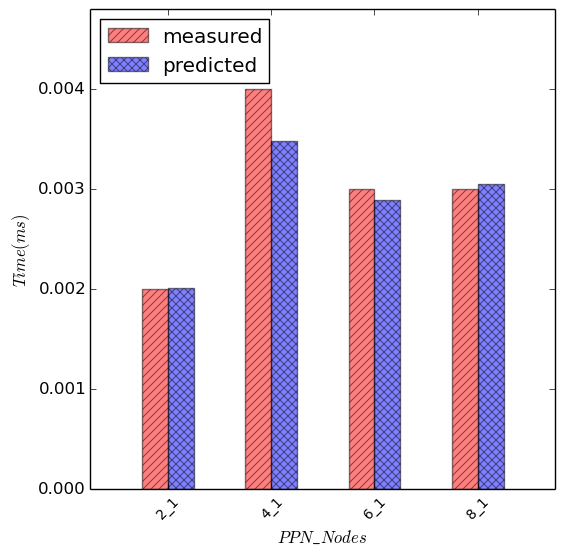
\includegraphics[width=\textwidth]{./images/broadcast/bcast_8.png}
        \caption{8B}
    \end{subfigure}
    \quad 
        \begin{subfigure}[b]{0.4\textwidth}
        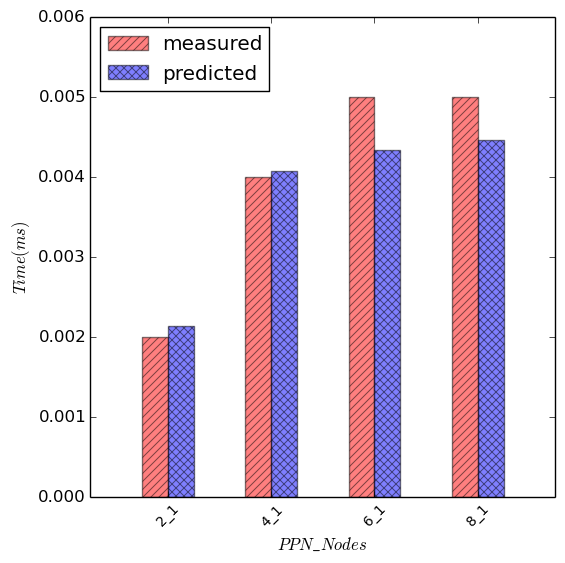
\includegraphics[width=\textwidth]{./images/broadcast/bcast_1024.png}
        \caption{1KiB}
    \end{subfigure}
    \quad
        \begin{subfigure}[b]{0.4\textwidth}
        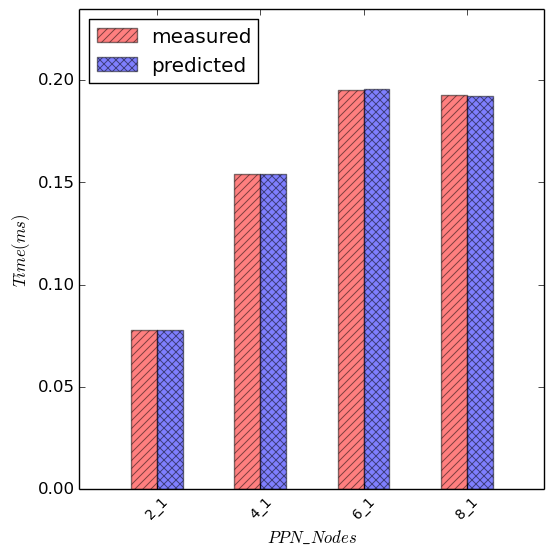
\includegraphics[width=\textwidth]{./images/broadcast/bcast_262144.png}
        \caption{256KiB}
    \end{subfigure}
    \quad
        \begin{subfigure}[b]{0.4\textwidth}
        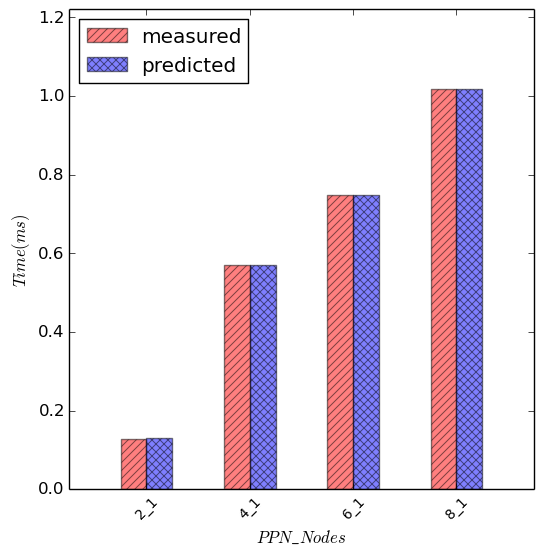
\includegraphics[width=\textwidth]{./images/broadcast/bcast_1048576.png}
        \caption{1MiB}
    \end{subfigure}

    \caption{Αποτελέσματα broadcast για σταθερό μέγεθος μηνύματος σε αρχιτεκτονική UMA}
        \label{fig:bcast_sizes}
\end{figure}
\begin{figure}[ht]
    \centering
     \captionsetup{justification=centering,margin=0cm,font=footnotesize}
    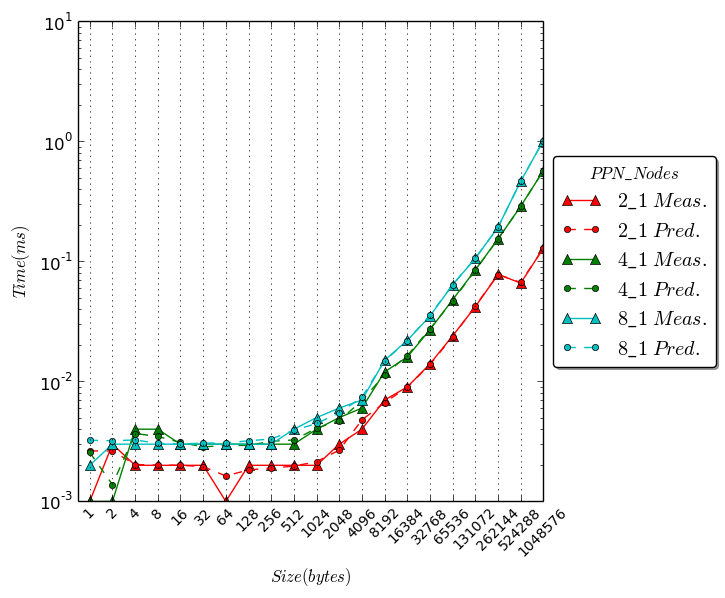
\includegraphics[width=0.7\textwidth]{./images/broadcast/bcast.png}
    \caption{Αποτελέσματα broadcast για μερικά configurations σε αρχιτεκτονική UMA}
    \label{fig:bcast_conf}
\end{figure}

\begin{figure}[H]
    \centering
    \captionsetup{justification=centering,margin=0cm,font=footnotesize}
    \begin{subfigure}[b]{0.4\textwidth}
        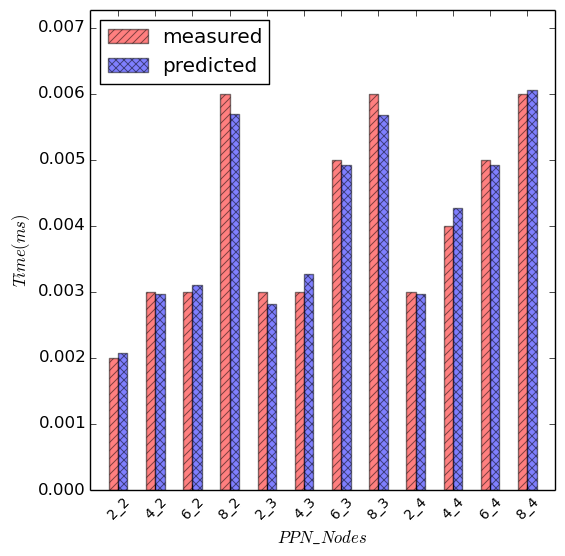
\includegraphics[width=\textwidth]{./images/broadcast_NUMA/bcast_8.png}
        \caption{8B}
    \end{subfigure}
    \quad 
        \begin{subfigure}[b]{0.4\textwidth}
        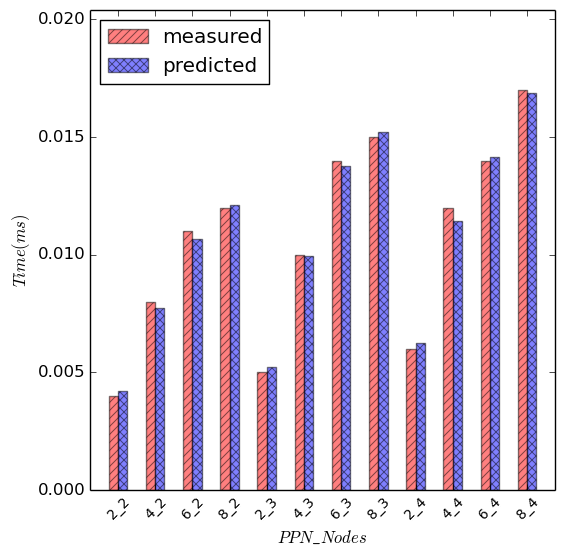
\includegraphics[width=\textwidth]{./images/broadcast_NUMA/bcast_1024.png}
        \caption{1KiB}
    \end{subfigure}
    \quad
        \begin{subfigure}[b]{0.4\textwidth}
        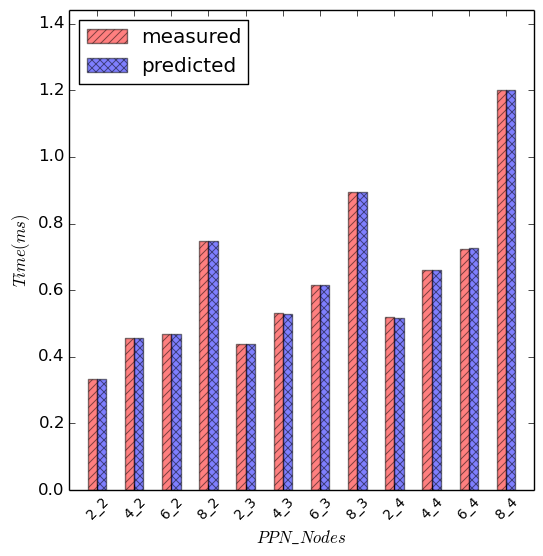
\includegraphics[width=\textwidth]{./images/broadcast_NUMA/bcast_262144.png}
        \caption{256KiB}
    \end{subfigure}
    \quad
        \begin{subfigure}[b]{0.4\textwidth}
        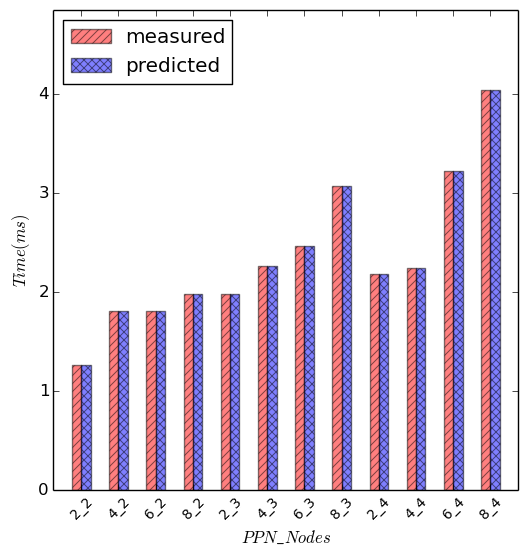
\includegraphics[width=\textwidth]{./images/broadcast_NUMA/bcast_1048576.png}
        \caption{1MiB}
    \end{subfigure}

    \caption{Αποτελέσματα broadcast για σταθερό μέγεθος μηνύματος σε αρχιτεκτονική NUMA}
        \label{fig:bcast_sizes_NUMA}
\end{figure}
\begin{figure}[ht]
    \centering
     \captionsetup{justification=centering,margin=0cm,font=footnotesize}
    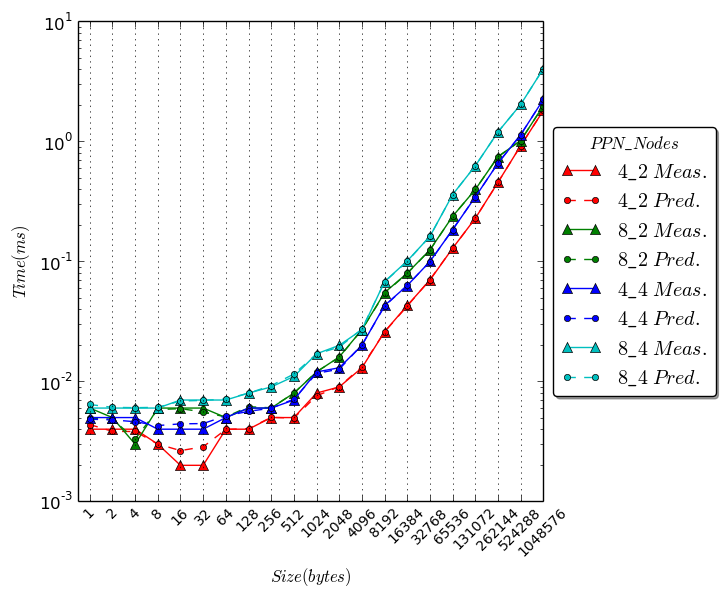
\includegraphics[width=0.7\textwidth]{./images/broadcast_NUMA/bcast.png}
    \caption{Αποτελέσματα broadcast για μερικά configurations σε αρχιτεκτονική NUMA}
    \label{fig:bcast_conf_NUMA}
\end{figure}

\section{Αllreduce}
\paragraph{}
Σε αυτή την υποενότητα καταπιανόμαστε με τα αποτελέσματα του  collective allreduce. Σε αντιστοιχία με τις προηγούμενες ενότητες, δίνονται τα αποτελέσματα για τις δύο αρχιτεκτονικές στα Σχήματα \ref{fig:allreduce_sizes}, \ref{fig:allreduce_conf}, \ref{fig:allreduce_sizes_NUMA} και \ref{fig:allreduce_conf_NUMA}. Ο κυριότερος λόγος που συμπεριλάβαμε τα αναλυτικά αποτελέσματα, είναι το Σχήμα \ref{fig:allreduce_conf_NUMA} και η συμπεριφορά του collective για μεγέθη μεταξύ 2KiB και 16KiB σε αρχιτεκτονική NUMA. Παρατηρούμε, ότι ο χρόνος επικοινωνίας, παρουσιάζει το φαινόμενο με την απότομη αύξηση του για μέγεθος 4KiB. Ωστόσο, με την περαιτέρω αύξηση του μεγέθους σε 16KiB η επικοινωνία διαρκεί λιγότερο σε σχέση με τα 4KiB για τα configurations με πολλά PPN. Επιβεβαιώσαμε ότι το παραπάνω συμβαίνει για κάθε εκτέλεση του allreduce αλλά δεν μπορέσαμε να προσδιορίσουμε τους λόγους που το προκαλούν. 

\paragraph{}
Γενικά, το allreduce ήταν το collective με την πιο παράξενη συμπεριφορά. Υπάρχουν περιπτώσεις, κυρίως σε μικρά μεγέθη μηνύματος, όπου με την αύξηση των δεσμευμένων πόρων ο χρόνος επικοινωνίας μειώνεται. Συγκεκριμένα, με την αύξηση των διεργασιών ανά κόμβο από 6 σε 8 παρατηρούμε μη μεταβολή ή μείωση του χρόνου επικοινωνίας για τα μηνύματα μικρότερα από 4KiB σε αρχιτεκτονική NUMA. 


\begin{figure}[ht]
    \centering
    \captionsetup{justification=centering,margin=0cm,font=footnotesize}
    \begin{subfigure}[b]{0.4\textwidth}
        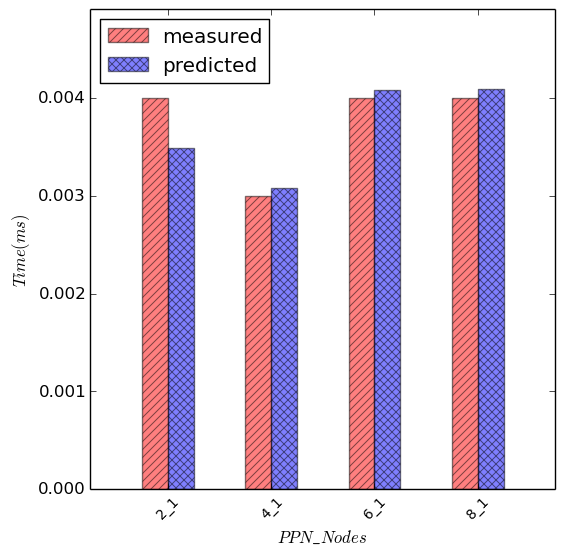
\includegraphics[width=\textwidth]{./images/allreduce/allreduce_8.png}
        \caption{8B}
    \end{subfigure}
    \quad 
        \begin{subfigure}[b]{0.4\textwidth}
        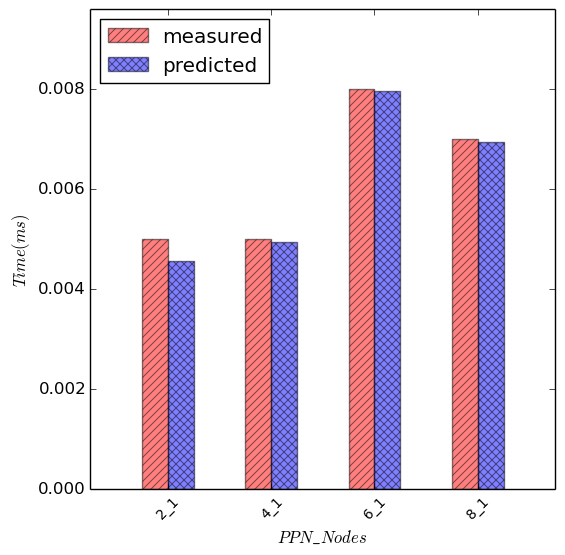
\includegraphics[width=\textwidth]{./images/allreduce/allreduce_1024.png}
        \caption{1KiB}
    \end{subfigure}
    \quad
        \begin{subfigure}[b]{0.4\textwidth}
        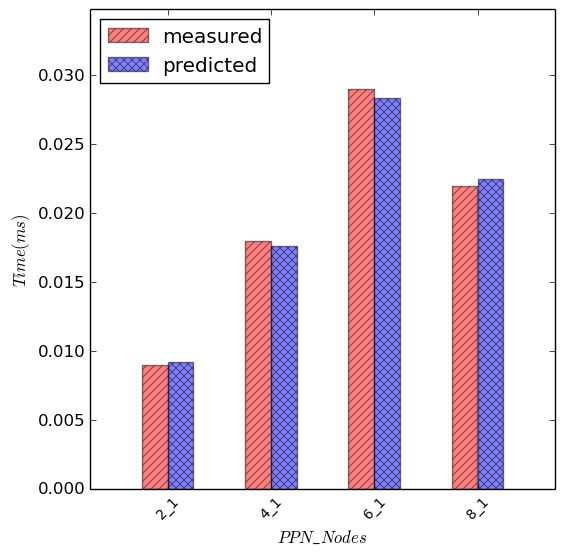
\includegraphics[width=\textwidth]{./images/allreduce/allreduce_4096.png}
        \caption{4KiB}
    \end{subfigure}
    \quad
        \begin{subfigure}[b]{0.4\textwidth}
        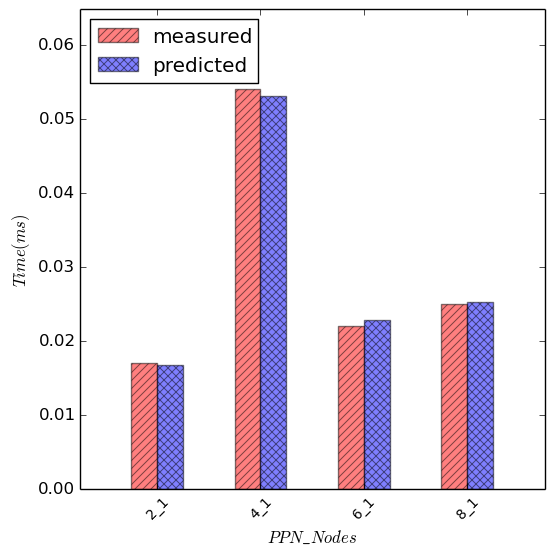
\includegraphics[width=\textwidth]{./images/allreduce/allreduce_16384.png}
        \caption{16KiB}
    \end{subfigure}

    \caption{Αποτελέσματα allreduce για σταθερό μέγεθος μηνύματος σε αρχιτεκτονική UMA}
        \label{fig:allreduce_sizes}
\end{figure}
\begin{figure}[ht]
    \centering
     \captionsetup{justification=centering,margin=0cm,font=footnotesize}
    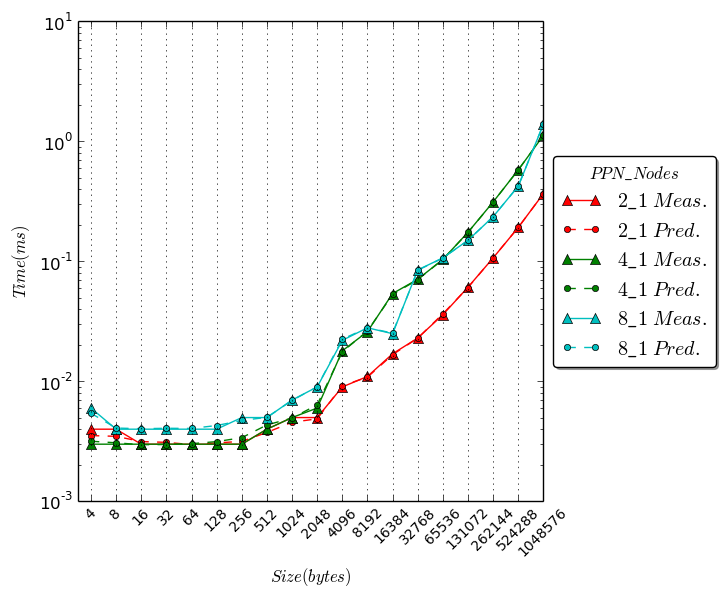
\includegraphics[width=0.7\textwidth]{./images/allreduce/allreduce.png}
    \caption{Αποτελέσματα allreduce για μερικά configurations σε αρχιτεκτονική UMA}
    \label{fig:allreduce_conf}
\end{figure}

\begin{figure}[H]
    \centering
    \captionsetup{justification=centering,margin=0cm,font=footnotesize}
    \begin{subfigure}[b]{0.4\textwidth}
        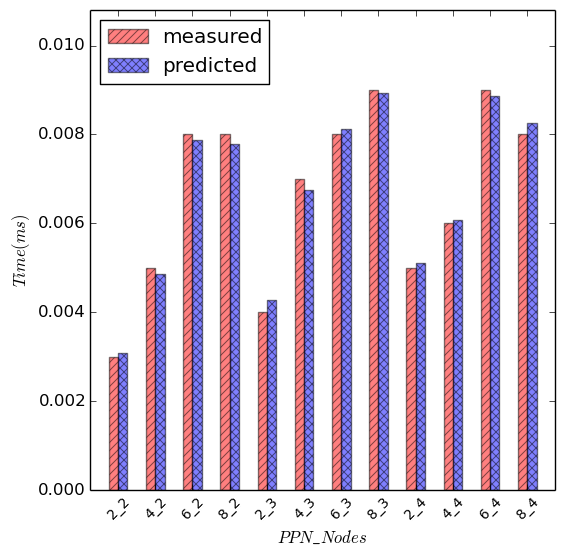
\includegraphics[width=\textwidth]{./images/allreduce_NUMA/allreduce_8.png}
        \caption{8B}
    \end{subfigure}
    \quad 
        \begin{subfigure}[b]{0.4\textwidth}
        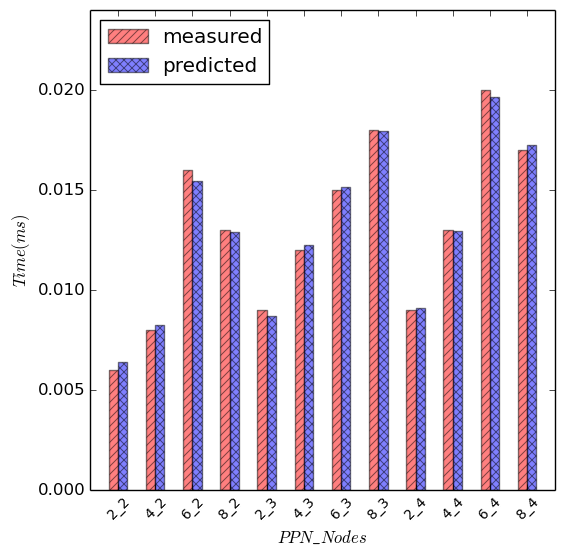
\includegraphics[width=\textwidth]{./images/allreduce_NUMA/allreduce_1024.png}
        \caption{1KiB}
    \end{subfigure}
    \quad
        \begin{subfigure}[b]{0.4\textwidth}
        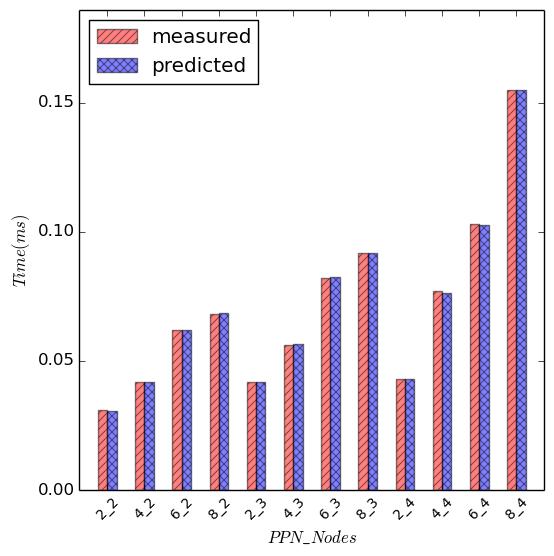
\includegraphics[width=\textwidth]{./images/allreduce_NUMA/allreduce_4096.png}
        \caption{4KiB}
    \end{subfigure}
    \quad
        \begin{subfigure}[b]{0.4\textwidth}
        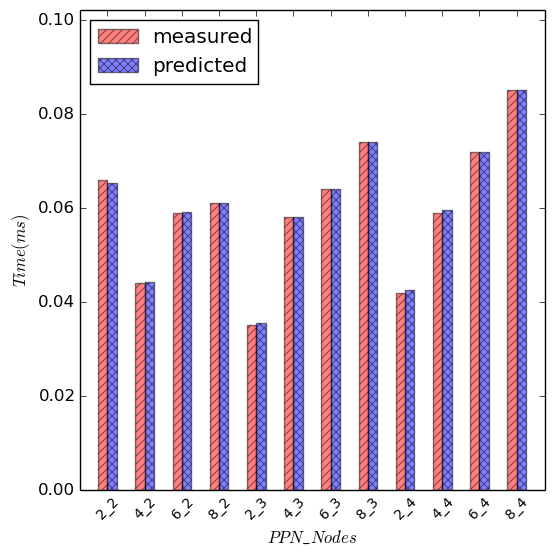
\includegraphics[width=\textwidth]{./images/allreduce_NUMA/allreduce_16384.png}
        \caption{16KiB}
    \end{subfigure}

    \caption{Αποτελέσματα allreduce για σταθερό μέγεθος μηνύματος σε αρχιτεκτονική NUMA}
        \label{fig:allreduce_sizes_NUMA}
\end{figure}
\begin{figure}[ht]
    \centering
     \captionsetup{justification=centering,margin=0cm,font=footnotesize}
    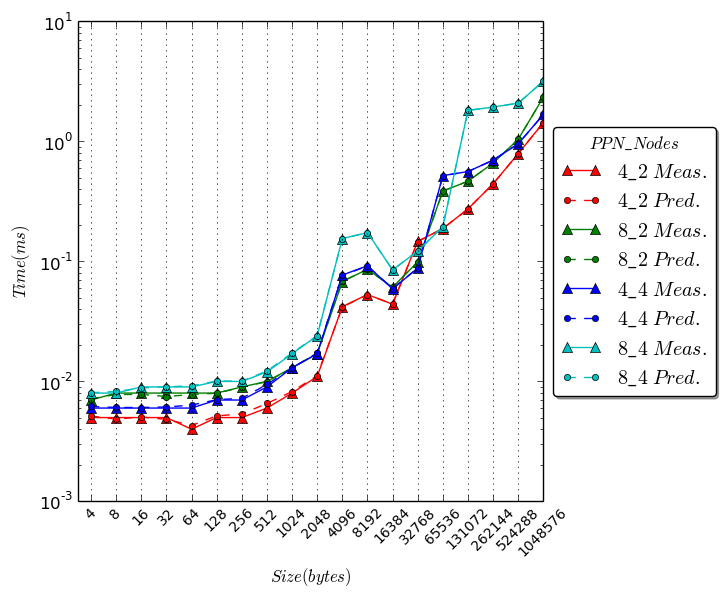
\includegraphics[width=0.7\textwidth]{./images/allreduce_NUMA/allreduce.png}
    \caption{Αποτελέσματα allreduce για μερικά configurations σε αρχιτεκτονική NUMA}
    \label{fig:allreduce_conf_NUMA}
\end{figure}

\section{Συγκεντρωτικά Αποτελέσματα για τα υπόλοιπα collectives}
Για λόγους πληρότητας στα επόμενα δύο σχήματα παραθέτουμε τις προβλέψεις για τα collectives που δεν παρουσιάζουμε τα αναλυτικά αποτελέσματα τους. Όπως και για τα προηγούμενα, παρατηρούμε ότι το μοντέλο επικοινωνίας προβλέπει τα σημεία εκπαίδευσης με μηδενικό σφάλμα.
\begin{figure}[H]
    \centering
    \captionsetup{justification=centering,margin=0cm,font=footnotesize}
    \begin{subfigure}[b]{0.4\textwidth}
        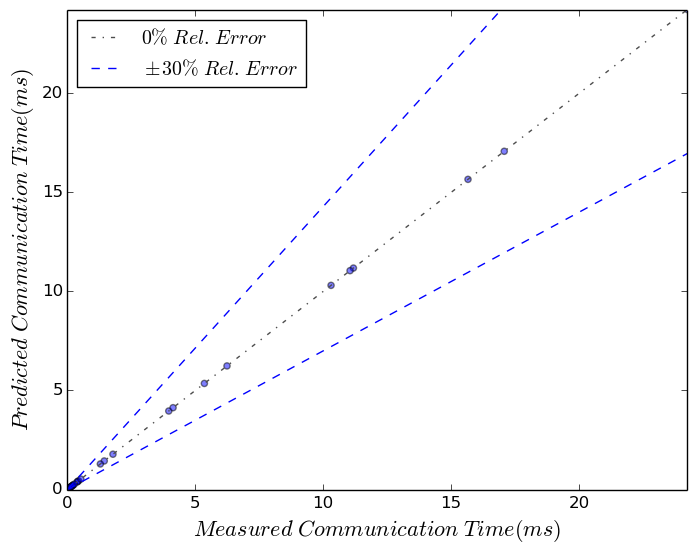
\includegraphics[width=\textwidth]{./images/all_UMA/gather.png}
        \caption{gather}
    \end{subfigure}
    \quad 
    \begin{subfigure}[b]{0.4\textwidth}
        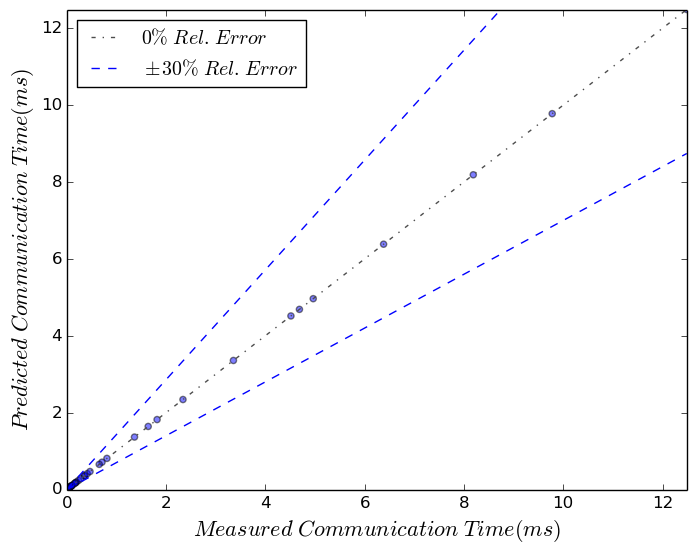
\includegraphics[width=\textwidth]{./images/all_UMA/reduce.png}
        \caption{reduce}
    \end{subfigure}
    \quad 
    \begin{subfigure}[b]{0.4\textwidth}
        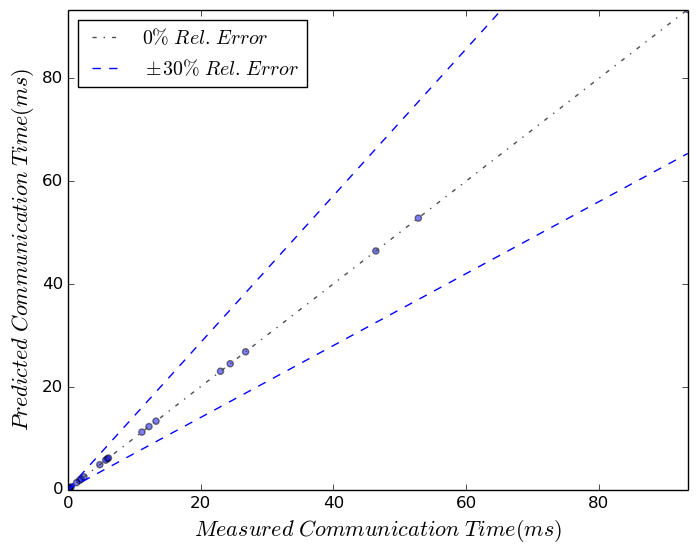
\includegraphics[width=\textwidth]{./images/all_UMA/allgather.png}
        \caption{allgather}
    \end{subfigure}
    \quad 
    \begin{subfigure}[b]{0.4\textwidth}
        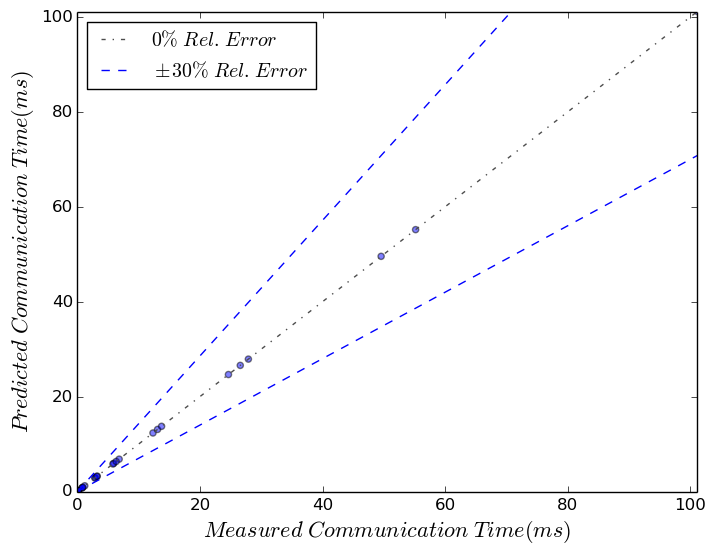
\includegraphics[width=\textwidth]{./images/all_UMA/alltoall.png}
        \caption{alltoall}
    \end{subfigure}


    \caption{Αποτελέσματα gather,reduce,allgather και alltoall για αρχιτεκτονική UMA}
\end{figure}

\begin{figure}[H]
    \centering
    \captionsetup{justification=centering,margin=0cm,font=footnotesize}
    \begin{subfigure}[b]{0.4\textwidth}
        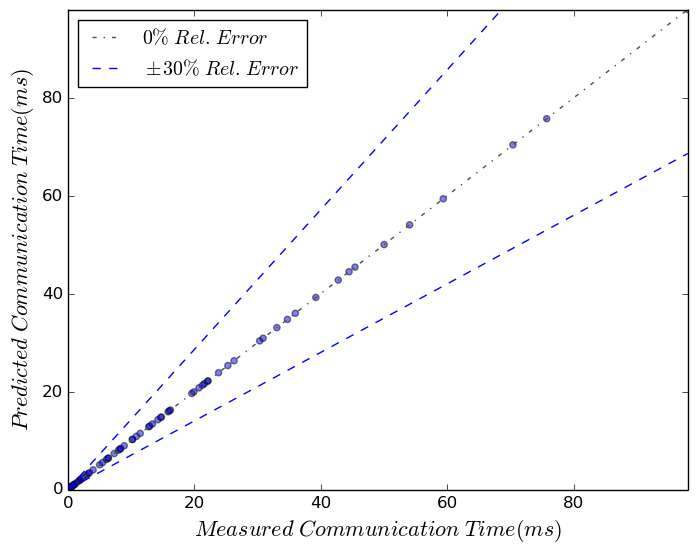
\includegraphics[width=\textwidth]{./images/all_NUMA/gather.png}
        \caption{gather}
    \end{subfigure}
    \quad 
    \begin{subfigure}[b]{0.4\textwidth}
        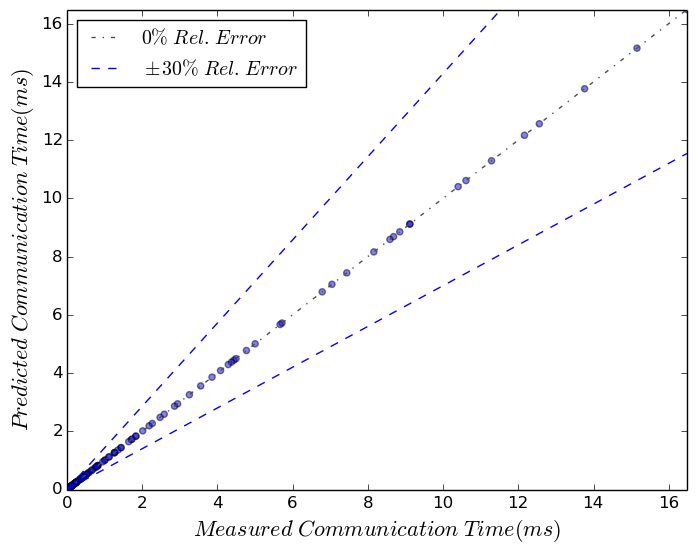
\includegraphics[width=\textwidth]{./images/all_NUMA/reduce.png}
        \caption{reduce}
    \end{subfigure}
    \quad 
    \begin{subfigure}[b]{0.4\textwidth}
        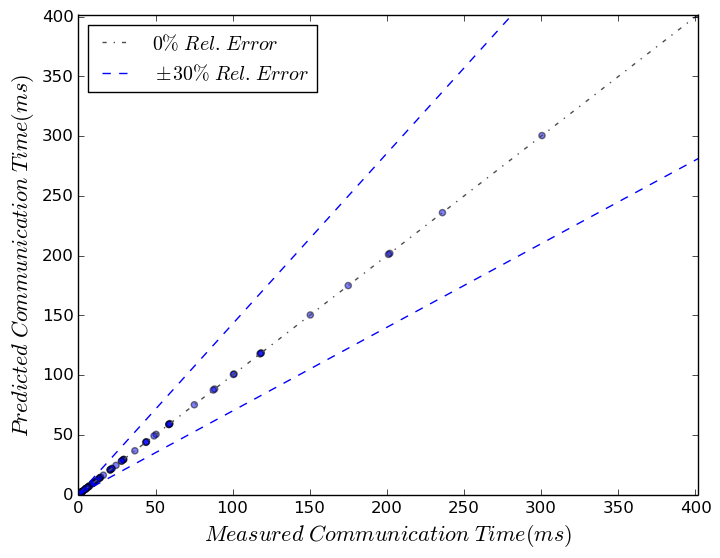
\includegraphics[width=\textwidth]{./images/all_NUMA/allgather.png}
        \caption{allgather}
    \end{subfigure}
    \quad 
    \begin{subfigure}[b]{0.4\textwidth}
        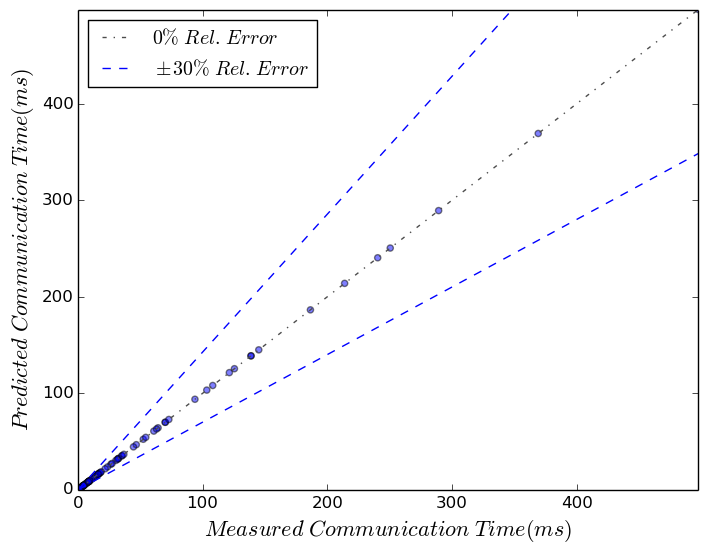
\includegraphics[width=\textwidth]{./images/all_NUMA/alltoall.png}
        \caption{alltoall}
    \end{subfigure}


    \caption{Αποτελέσματα gather,reduce,allgather και alltoall για αρχιτεκτονική UMA}
\end{figure}

\section{Αποτελέσματα εφαρμογής LULESH}
\paragraph{}
Όπως αναφέραμε πιο πάνω, για την πειραματική αξιολόγηση των μοντέλων στηριχτήκαμε στο collective allreduce που εκτελεί η εφαρμογή LULESH επαναληπτικά.  Χρησιμοποιήθηκαν οι ίδιες μετρικές αξιολόγησης με την point-to-point επικοινωνία ενώ, ο μετρούμενος χρόνος επικοινωνίας υπολογίζεται αθροιστικά πάνω από τις επαναλήψεις. H τελική πρόβλεψη είναι το γινόμενο του αριθμού των επαναλήψεων με την πρόβλεψη του χρόνου για μία επανάληψη. Και πάλι, ο αλγόριθμος επιβλεπόμενης μάθησης για την εκπαίδευση των μοντέλων ήταν ο \textit{GBTR}, του οποίου  διατρέξαμε τις παραμέτρους και παρουσιάζουμε τις καλύτερες δυνατές προβλέψεις. 
\subsection{Αρχιτεκτονική UMA}
\paragraph{}
Στο Σχήμα \ref{fig:coll_UMA} δίνονται οι προβλέψεις, η κατανομή του απόλυτου σχετικού σφάλματος, οι παράμετροι εκπαίδευσης του μοντέλου και οι τιμές των μετρικών αξιολόγησης σε αρχιτεκτονική UMA. Οφείλουμε να αναφέρουμε, ότι το μέγεθος του χωρίου δεν επηρεάζει το μέγεθος των δεδομένων που θα δοθούν σαν είσοδο στο collective. Σε κάθε περίπτωση, το collective εκτελεί allreduce για ένα αριθμό διπλής ακρίβειας, 8 bytes και ο χρόνος επικοινωνίας είναι σχεδόν ανεπηρέαστος από το μέγεθος του χωρίου. Η ακρίβεια των προβλέψεων ήταν συγκρίσιμη με αυτή της point-to-point επικοινωνίας. Από τη γραφική ξεχωρίζει, η εκτόξευση του μετρούμενου χρόνου επικοινωνίας για μέγεθος χωρίου $100^3$. Εκτελέσαμε την εφαρμογή αρκετές φορές και παρατηρήσαμε ότι η απότομη αύξηση αυτή δεν λαμβάνει χώρα πάντα για το συγκεκριμένο μέγεθος χωρίου αλλά έχει τη τάση να εμφανίζεται για κάποιο από τα μεγαλύτερα. Όπως αναφέραμε πιο πάνω, η υλοποίηση του allreduce απαιτεί τη δέσμευση 2 buffers 8KiB από κάθε διεργασία που μετέχει στη διαδικασία, ανεξαρτήτως του μεγέθους των δεδομένων που αφορά το collective. Όμως, καθώς το μέγεθος του χωρίου μεγαλώνει, οι απαιτήσεις της εφαρμογής σε μνήμη αυξάνουν. Σαν αποτέλεσμα, φαινόμενα που δυσχεραίνουν τη δέσμευση μνήμης, όπως κατακερματισμός του σωρού, εισάγουν καθυστέρηση στην εκτέλεση του collective, που εμείς υποθέτουμε ότι αναλώνει χρόνο μόνο για επικοινωνία. Τέλος, όλα τα υπόλοιπα σημεία παρουσιάζουν σφάλμα μικρότερο του 30\%.
\begin{figure}[H]
    \centering
    \captionsetup{justification=centering,margin=0cm,font=footnotesize}
    \begin{subfigure}[b]{0.47\textwidth}
        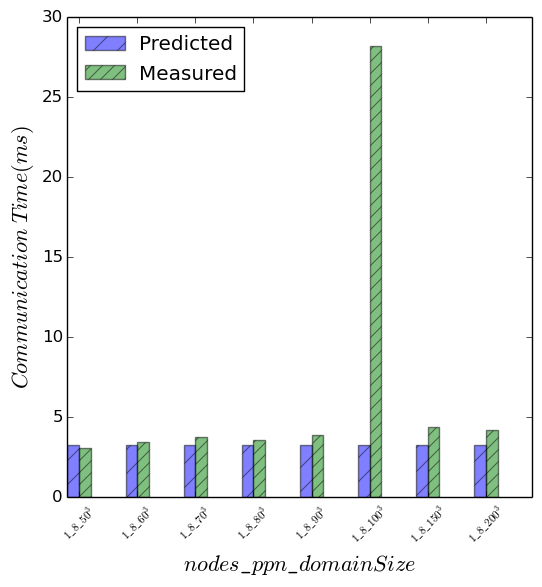
\includegraphics[width=\textwidth]{./images/coll_UMA/res.png}
        \caption{Αποτελέσματα}
    \end{subfigure}
    \quad %add desired spacing between images, e. g. ~, \quad, \qquad, \hfill etc. 
      %(or a blank line to force the subfigure onto a new line)
    \begin{subfigure}[b]{0.47\textwidth}
        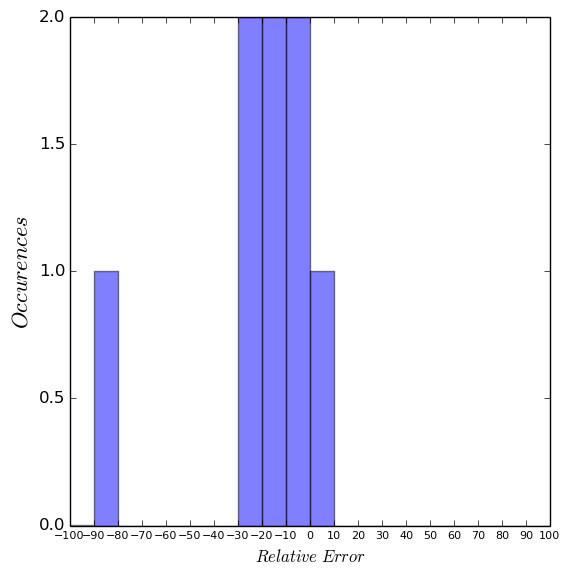
\includegraphics[width=\textwidth]{./images/coll_UMA/err_dist.png}
        \caption{Κατανομή Σφάλματος}
    \end{subfigure} 
    \\[0.2cm]
    \begin{subfigure}[b]{\textwidth}
   	 	\scriptsize
		\begin{tabular}{c||c|c|c|c|c}
			\textbf{Παράμετρος} & n\_estimators & learning\_rate & max\_depth & min\_samples\_leaf & min\_samples\_split \\
			\textbf{Τιμή}       &       200        &  0.025               & 8          &  1                  &    2
		\end{tabular}
		\caption{Παράμετροι Μοντέλου}
    \end{subfigure}
    \\[0.2cm]
    \begin{subfigure}[b]{\textwidth}
    		\centering
   	 	\scriptsize
		\begin{tabular}{c||c|c|c}
			\textbf{Μετρική} & $RCC$ &   $avg(|e|)$ & $Pred_{0.3}$  \\
			\textbf{Τιμή}  &  $0.857$   &      $23.56\%
			$        &  $88\%$                                         
		\end{tabular}
		\caption{Μετρικές Αξιολόγησης}
    \end{subfigure}
            \caption{Αποτελέσματα, κατανομή σφάλματος, παράμετροι εκπαίδευσης και μετρικές αξιολόγησης για την εφαρμογή LULESH σε αρχιτεκτονική UMA για collective επικοινωνία}
    \label{fig:coll_UMA}
\end{figure}

\subsection{Αρχιτεκτονική NUMA}
Στο Σχήμα \ref{fig:coll_NUMA} φαίνονται τα αντίστοιχα αποτελέσματα για την NUMA αρχιτεκτονική. Παρατηρούμε ότι υπάρχουν αρκετές μεταβολές στους χρόνους επικοινωνίας παρόλο που περιμέναμε ότι θα είναι ανεξάρτητοι από το μέγεθος του χωρίου της εφαρμογής. Για κάποια από τα μεγαλύτερα μεγέθη χωρίων, η αύξηση φτάνει μέχρι και σε διπλασιασμό του χρόνου επικοινωνίας. Ο λόγος που ο χρόνος επικοινωνίας του allreduce είναι τόσο μεταβαλλόμενος είναι και πάλι ο θόρυβος που εισάγεται στις μετρήσεις από το λειτουργικό με τη δέσμευση των δύο buffers. Οφείλουμε να ομολογήσουμε, ότι το μοντέλο επικοινωνίας που αναπτύξαμε, αδυνατεί να προβλέψει τέτοια φαινόμενα. Δεν συμπεριλάβαμε μετρικές που να συσχετίζουν πόσο απαιτητική σε μνήμη είναι η εφαρμογή με το χρόνο επικοινωνίας, ούτε είχαμε δείγματα στο testing set που να εμφανίζουν τέτοια φαινόμενα. Παρόλα αυτά, σε μελλοντικές υλοποιήσεις του MPI μπορεί το μέγεθος των εσωτερικών buffers να ορίζεται από το μέγεθος των δεδομένων που ανταλλάσσονται ή να γίνεται επαναχρησιμοποίηση των buffers. Σε τέτοια περίπτωση τα φαινόμενα αυτά θα είναι αμελητέα και η μεθοδολογία μας θα εμφανίζει ακόμα καλύτερα αποτελέσματα. Παρόλα αυτά η ακρίβεια του μοντέλου μας είναι αρκετά υψηλή, με το μέσο απόλυτο σφάλμα να περιορίζεται στα 20.18\% και τη τιμή του $Pred_{0.3}$ να αγγίζει τα 75\%. 

\begin{figure}[H]
    \centering
    \captionsetup{justification=centering,margin=0cm,font=footnotesize}
    \begin{subfigure}[b]{0.47\textwidth}
        \includegraphics[width=\textwidth]{./images/coll_NUMA/res.png}
        \caption{Αποτελέσματα}
    \end{subfigure}
    \quad %add desired spacing between images, e. g. ~, \quad, \qquad, \hfill etc. 
      %(or a blank line to force the subfigure onto a new line)
    \begin{subfigure}[b]{0.47\textwidth}
        \includegraphics[width=\textwidth]{./images/coll_NUMA/Err_Dist.png}
        \caption{Κατανομή Σφάλματος}
    \end{subfigure} 
    \\[0.2cm]
    \begin{subfigure}[b]{\textwidth}
   	 	\scriptsize
		\begin{tabular}{c||c|c|c|c|c}
			\textbf{Παράμετρος} & n\_estimators & learning\_rate & max\_depth & min\_samples\_leaf & min\_samples\_split \\
			\textbf{Τιμή}       &       200        &  0.03               & 10          &  1                  &    2
		\end{tabular}
		\caption{Παράμετροι Μοντέλου}
    \end{subfigure}
    \\[0.2cm]
    \begin{subfigure}[b]{\textwidth}
    		\centering
   	 	\scriptsize
		\begin{tabular}{c||c|c|c}
			\textbf{Μετρική} & $RCC$ &   $avg(|e|)$ & $Pred_{0.3}$  \\
			\textbf{Τιμή}  &  $0.808$   &      $20.179\%
			$        &  $75\%$                                         
		\end{tabular}
		\caption{Μετρικές Αξιολόγησης}
    \end{subfigure}
            \caption{Αποτελέσματα, κατανομή σφάλματος, παράμετροι εκπαίδευσης και μετρικές αξιολόγησης για την εφαρμογή LULESH σε αρχιτεκτονική NUMA για collective επικοινωνία. }
    \label{fig:coll_NUMA}
\end{figure}
\section{Σύγκριση αποτελεσμάτων με βάση την απεικόνιση των διεργασιών στους πόρους}
Σε όλα τα αποτελέσματα μας μέχρι τώρα, η απεικόνιση των διεργασιών στους πόρους του μηχανήματος γινόταν bycore, δηλαδή MPI διεργασίες με γειτονικά αναγνωριστικά τοποθετούνταν στον ίδιο κόμβο. Παραδείγματος χάρη, για 4 κόμβους και 4 PPN οι διεργασίες με αναγνωριστικά 0-3 εκτελούνταν στον πρώτο κόμβο, με αναγνωριστικά 4-7 στο δεύτερο και ούτω καθεξής. Θέλαμε να εξετάσουμε κατά πόσο ο χρόνος εκτέλεσης επηρεάζεται σε περίπτωση που η απεικόνιση γινόταν bynode, δηλαδή MPI διεργασίες με γειτονικά αναγνωριστικά να τοποθετηθούν σε γειτονικούς NUMA κόμβους. Έτσι, εκτελέσαμε τα benchmarks για όλα τα collectives και για τις δύο απεικονίσεις με τα αποτελέσματα να δίνονται στο Σχήμα \ref{fig:bycore_vs_bynode}. 
\paragraph{}
Με την αλλαγή της απεικόνισης παρατηρήσαμε σημαντικές διαφορές. Τα collectives scatter και gather φαίνεται να επηρεάζονται αρνητικά από τη bynode κατανομή, αφού σε κάθε περίπτωση ο χρόνος επικοινωνίας είναι μικρότερος με τη bycore. Αντίθετα, τα υπόλοιπα collectives επωφελούνται από τη bynode απεικόνιση με περίπου 30\% μείωση του χρόνου επικοινωνίας. Καθώς η επίδραση της αλλαγής της απεικόνισης διαφέρει από collective σε collective είναι προφανές ότι η υλοποίηση του εκάστοτε collective είναι ένας από τους λόγους που παρατηρούμε το παραπάνω φαινόμενο. Επιπλέον, καθώς το OpenMPI δεν λαμβάνει υπόψη του την απεικόνιση των διεργασιών στους πόρους, οι ανταλλαγές μηνυμάτων, από τη σκοπιά του OpenMPI που συμβαίνουν στις δύο περιπτώσεις είναι οι ίδιες. Σε μια ιδανική υλοποίηση, όπου το περιβάλλον εκτέλεσης του MPI θα λάμβανε υπόψη την αρχιτεκτονική του συστήματος για να βελτιστοποιήσει την επικοινωνία, δεν θα είχαμε ανάλογης κλίμακας μεταβολή στους χρόνους επικοινωνίας. 
\paragraph{}
Οφείλουμε να ομολογήσουμε ότι αυτό αποτελεί και τη μεγαλύτερη αδυναμία της μεθοδολογίας μας για τη collective επικοινωνία η οποία θα δώσει τις ίδιες τιμές στα χαρακτηριστικά για τα δύο mappings με αποτέλεσμα μεγάλα σφάλματα σε πιθανές προβλέψεις όπου τα mappings διαφέρουν. 
\paragraph{}
Επιπρόσθετα, εξετάσαμε την επίδραση της αλλαγής της διεργασίας ρίζας στο χρόνο επικοινωνίας των collectives που μας το επέτρεπαν. Στο Σχήμα \ref{fig:root}  παραθέτουμε τα αποτελέσματα για το collective reduce και 32 διεργασίες. Τα μεγαλύτερα μηνύματα δαπανούν τον ίδιο χρόνο επικοινωνίας, ενώ παρατηρούμε μία μικρή απόκλιση στο χρόνο επικοινωνίας όταν η διεργασία ρίζα τοποθετείται στο κόμβο 0. Αφού καθώς το μέγεθος αυξάνει οι χρόνοι επικοινωνίας ταυτίζονται, η μικρή απόκλιση που παρατηρήσαμε για τα μικρότερα μηνύματα οφείλεται και πάλι σε θόρυβο που εισάγει το λειτουργικό σύστημα. Πιθανότατα, το λειτουργικό σύστημα χρησιμοποιεί πόρους από τον κόμβο 0. 

\begin{figure}[ht]
    \centering
     \captionsetup{justification=centering,margin=0cm,font=footnotesize}
    \includegraphics[width=0.7\textwidth]{./images/root.png}
    \caption{Χρόνοι επικοινωνίας για το collective reduce με τη μεταβολή της διεργασίας ρίζας}
    \label{fig:root}
\end{figure}

\begin{figure}[ht]
    \centering
    \begin{subfigure}[b]{0.40\textwidth}
        \includegraphics[width=\textwidth]{./images/bycore_vs_bynode/scatter.png}
        \caption{scatter}
    \end{subfigure}
    \quad 
     \begin{subfigure}[b]{0.40\textwidth}
        \includegraphics[width=\textwidth]{./images/bycore_vs_bynode/gather.png}
        \caption{gather}
    \end{subfigure}
    \quad
    \begin{subfigure}[b]{0.40\textwidth}
        \includegraphics[width=\textwidth]{./images/bycore_vs_bynode/reduce.png}
        \caption{reduce}
    \end{subfigure}
    \quad 
     \begin{subfigure}[b]{0.40\textwidth}
        \includegraphics[width=\textwidth]{./images/bycore_vs_bynode/bcast.png}
        \caption{broadcast}
    \end{subfigure}
     \quad
    \begin{subfigure}[b]{0.40\textwidth}
        \includegraphics[width=\textwidth]{./images/bycore_vs_bynode/allreduce.png}
        \caption{allreduce}
    \end{subfigure}
    \quad 
     \begin{subfigure}[b]{0.40\textwidth}
        \includegraphics[width=\textwidth]{./images/bycore_vs_bynode/allgather.png}
        \caption{allgather}
    \end{subfigure}
    \quad 
     \begin{subfigure}[b]{0.40\textwidth}
        \includegraphics[width=\textwidth]{./images/bycore_vs_bynode/alltoall.png}
        \caption{alltoall}
    \end{subfigure}
    \caption{Αποτελέσματα για κατανομή bycore και bynode}
    \label{fig:bycore_vs_bynode}
\end{figure}


	
